% !TEX root = ../Yan Hao-Dissertation.tex

\chapter{Introduction} \label{chapter1:Introduction}

\section{About Fiscal Federalism}

Many countries, regardless of their explicit federal system in terms of political structure, face issues related to the hierarchical structure of governments, which results in an unequal distribution of political and economic powers. Fiscal federalism is distinguished by the potential misalignment of expenditure responsibilities and revenue assignments. Fiscal federalism is a form of fiscal decentralization that is widely recognized as a more efficient way to provide public goods and services, particularly in large and complex countries with multiple levels of administrative institutions. Hayek \cite{hayek2009use} argued that local governments are better positioned to understand local needs and preferences, and therefore to provide appropriate public goods and services. Stigler \cite{stigler1998tenable} built on Hayek's insights and argued for the necessity of protecting the funding ability of subnational governments. Tiebout \cite{tiebout1956pure} developed a theoretical framework to show that voting with one's feet can ensure that public goods supply matches local needs. He also demonstrated that competition among local governments can lead to improved administrative efficiency. Tiebout's theory seems get supported by the actual data showed in Table \ref*{Table 1.1}, which potentially reflects the difference of tax burden preference of different states. These foundational insights form the basis for much of the research on the advantages of fiscal federalism.
\begin{table}[H]
  \centering
  \caption{Effective Tax Revenue in America}
  \begin{tabular}{p{9.43em}lll}
    \toprule
    State                & \multicolumn{1}{p{8.145em}}{State and Local Taxes (\$ billions)} & \multicolumn{1}{p{7.43em}}{Personal Income (\$ billions)} & \multicolumn{1}{p{9.93em}}{Effective Tax Rate} \\
    \midrule
    New York             & \multicolumn{1}{c}{177.8}                                        & \multicolumn{1}{c}{1,281.10}                              & \multicolumn{1}{c}{13.90\%}                    \\
    District of Columbia & \multicolumn{1}{c}{7.5}                                          & \multicolumn{1}{c}{55.5}                                  & \multicolumn{1}{c}{13.40\%}                    \\
    North Dakota         & \multicolumn{1}{c}{5}                                            & \multicolumn{1}{c}{39.5}                                  & \multicolumn{1}{c}{12.70\%}                    \\
    Hawaii               & \multicolumn{1}{c}{9.5}                                          & \multicolumn{1}{c}{75.4}                                  & \multicolumn{1}{c}{12.60\%}                    \\
    Vermont              & \multicolumn{1}{c}{3.8}                                          & \multicolumn{1}{c}{32.6}                                  & \multicolumn{1}{c}{11.70\%}                    \\
    \midrule
    United States Total  & \multicolumn{1}{c}{1,652.80}                                     & \multicolumn{1}{c}{16,820.30}                             & \multicolumn{1}{c}{9.80\%}                     \\
    \midrule
    Alabama              & \multicolumn{1}{c}{16.4}                                         & \multicolumn{1}{c}{198.9}                                 & \multicolumn{1}{c}{8.30\%}                     \\
    Oklahoma             & \multicolumn{1}{c}{13.9}                                         & \multicolumn{1}{c}{174.4}                                 & \multicolumn{1}{c}{8.00\%}                     \\
    \midrule
    \multicolumn{4}{p{34.935em}}{\textit{Source:U.S. Census Bureau Dataset}}                                                                                                                             \\
  \end{tabular}%
  \label{Table 1.1}%
\end{table}%

In this chapter, I provide an overview of the fiscal federalism structure, focusing on the revenue sources for different levels of government, public service responsibilities, and the financial connection between central and subnational governments, as illustrated in Figure \ref*{Figure 1.1}. Specifically, central and local governments have distinct methods for generating revenue and supplying public goods and services, and the central government join public goods provision either through transfer payments, known as intergovernmental transfers or joint provision, allowing subnational jurisdictions to maintain necessary public goods and services while governments in two layers expressing their political intentions and concerns in this process.

\begin{figure}[H]
  \centering
  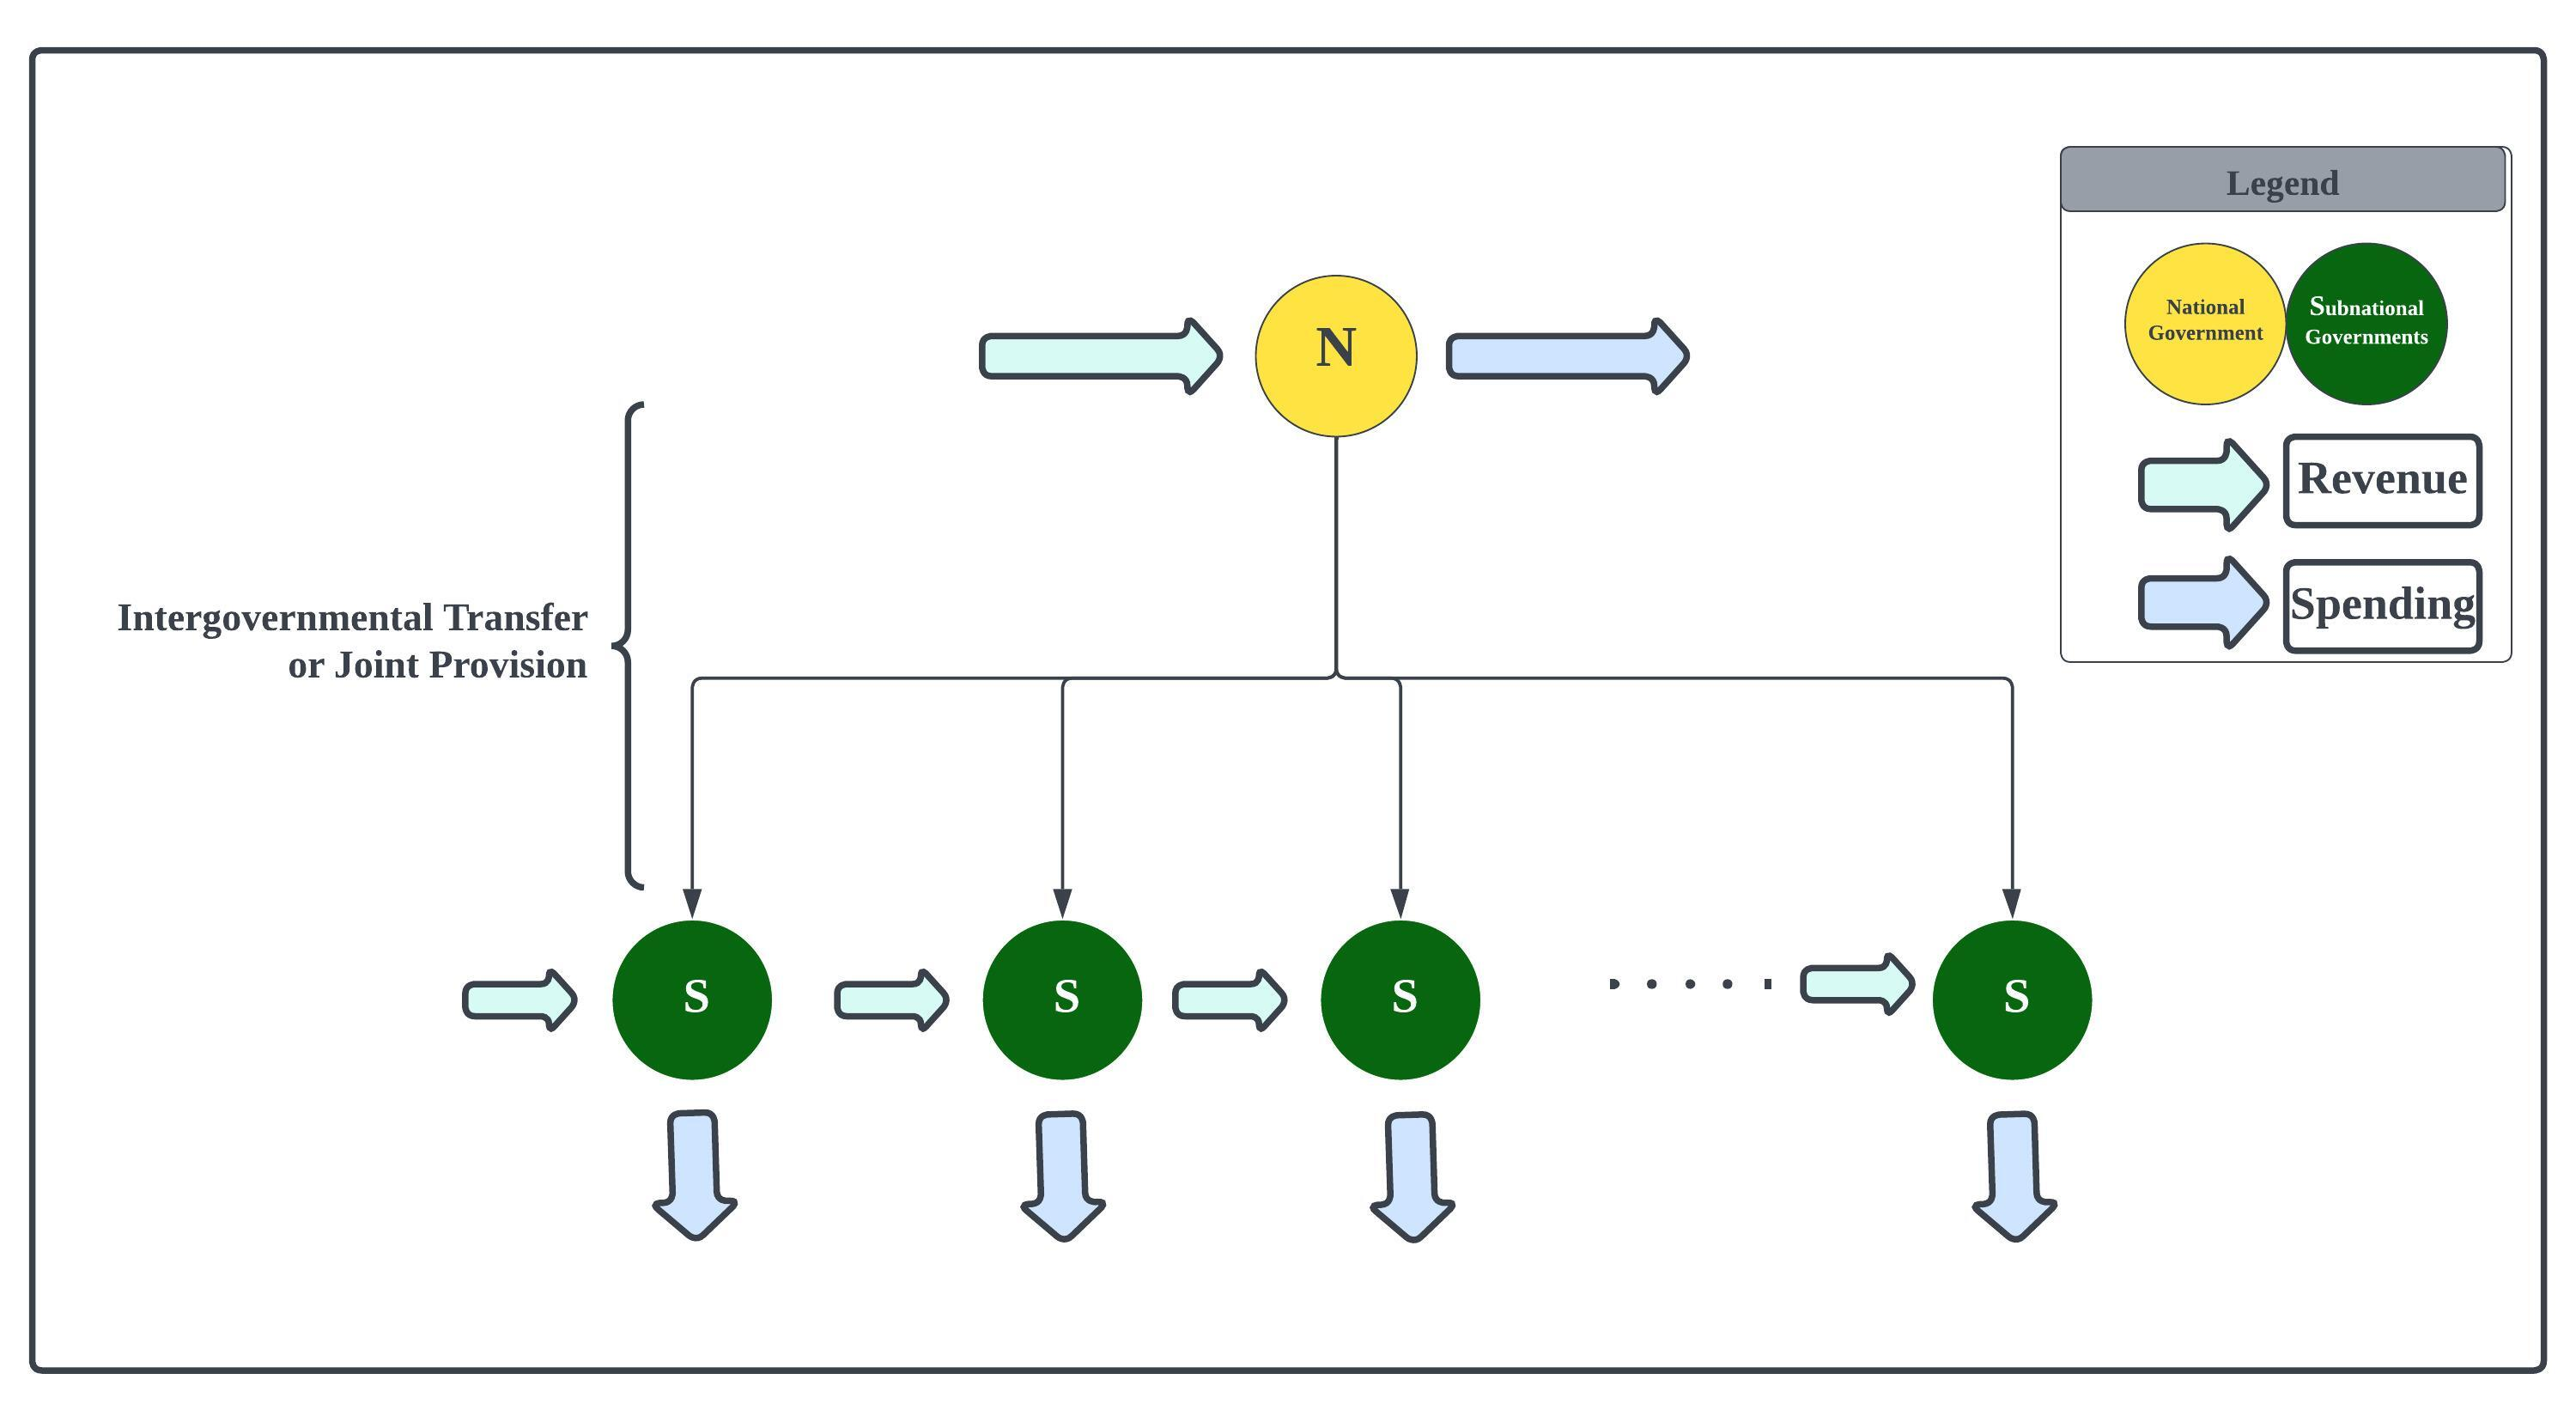
\includegraphics[scale=0.6]{Chapter-1/Figures/fiscal federalism.jpeg}
  \caption[Fiscal Federalism Structure]{Fiscal Federalism Structure
    \texttt{} }
  \label{Figure 1.1}
\end{figure}

For the following part of this chapter, I'll briefly summarize the literature on the evaluation of fiscal federalism, what are the topics that are commonly mentioned in related research.  After that I'll give a basic introduction about the fiscal federalism structure in USA, to be more specific, I'll talk about the revenue and responsibilities of different levels of governments, and fiscal interaction between different levels of governments.

\subsection{The Evaluation of the Fiscal Federalism System}
Even within the topic of fiscal federalism, the fiscal federalism structures in different countries have different content and features, needless to say, they show different impact in public goods and services supplying. Like I mentioned in Chapter 1, it's hard and nearly impossible to find a perfect stick yard criterion to compare fiscal federalism in different countries. I'll try to explain and get a comprehensive way to evaluate fiscal federalism. Literature about fiscal federalism can be roughly divided into two groups. First-generation theory of fiscal federalism concentrate on the fiscal structure itself, focusing on the efficiency of federalism in collecting revenue and offering responsibilities, and whether the revenue-responsibility combination perform well in public goods supply. Coming to second-generation theory of fiscal federalism, scholars get interested in the effect of fiscal federalism on other area such as the effect on economic development.

\subsubsection{First-Generation Theory of Fiscal Federalism}

Evaluating the efficiency of fiscal structures is a common approach to assessing their reasonableness. Pareto efficiency, which requires that resources be allocated in a manner that cannot make anyone better off without making someone else worse off, is widely accepted as a standard for evaluation \cite{pareto2014manual}. Scholars have identified three economic factors useful in evaluating fiscal structures: externalities, information complexity, and incentive compatibility. Oates \cite{oates1972fiscal} proposed that governments and residents of a jurisdiction should bear the costs of negative externalities and receive payment for positive externalities. Olson \cite{olson1993dictatorship} argued that the "free rider" problem could be resolved by making jurisdictions and beneficiary areas identical, achieving an equilibrium in which marginal costs equal marginal benefits. One example of an efficiency consideration in the United States' fiscal federalism structure is the revenue structure for individual taxes, as shown in Table \ref*{Table 1.2}. To minimize behavioral distortions and improve efficiency, individual income taxes, which are easy to move across jurisdictions, are mainly collected by federal and state governments, allowing individuals to be indifferent about where they live and pay taxes.

% Table generated by Excel2LaTeX from sheet 'Sheet1'
\begin{table}[htbp]
  \centering
  \caption{. Percentage Composition of Tax Revenue by Government Level}
  \begin{tabular}{lccc}
    \toprule
    \multicolumn{1}{c}{Type} & Federal & State   & Local   \\
    \midrule
    Individual income        & 51.80\% & 37.20\% & 4.70\%  \\
    Corporate income         & 6.90\%  & 4.70\%  & 1.10\%  \\
    Other taxes              & 41.20\% & 58.10\% & 94.20\% \\
    \bottomrule
  \end{tabular}%
  \label{Table 1.2}%
\end{table}%


Besides, information complexity is an important consideration in evaluating fiscal federalism structure. Basing their work on the earlier contributions of Hayek and Tiebout, Bseley et al \cite{2003Centralized} developed a political economy model to simulate the decision-making process in a democratic country. They emphasized the advantage of local government in public goods supplying and introduced insensitivity of central government into their model. Information communication is also important, with local governments having better knowledge of local residents' needs and their behavior being better perceived by local residents. Decentralized fiscal federalism structures put local governments under supervision, as noted by Dethier \cite{martinez2003fiscal} and based on Tiebout's voting on feet framework. Baicker \cite{baicker2005spillover} introduced a horizontal competition structure with multiple local governments and states that enables local residents to evaluate local governments' efficiency in public goods supply under a yardstick competition framework. This information transparency can push local governments to improve their performance.

Finally, a well-designed fiscal structure should satisfy the criterion of incentive compatibility. Incentive compatibility is a game theory concept introduced by Leonid Hurwicz \cite{hurwicz1973design} that requires a mechanism to be designed such that each participant can achieve the best outcome for themselves by acting truthfully. In public administration and public economics, incentive compatibility has become an important criterion for evaluating the quality of fiscal federalism. Proper fiscal federalism settings can motivate local governments to efficiently provide public goods. For example, Eckstein \cite{eckstein1958water} argues that the proper combination of funding resources and responsibilities can motivate organizations, including local governments, to work hard and provide public goods efficiently, since working hard with efficiency in public goods supplying is an weakly dominate strategy and could attract more residents and increase more public funding resource. Under the impact of incentive compatibility theory, scholars generally assume that local governments aim to maximize local fiscal revenue in fiscal federalism administration process. (Baretti, Bucovetsky,Dahlby,Jha) \cite{baretti2002tax,bucovetsky2006efficiency,dahlby2011marginal,jha2000tax}.

The first-generation theory of fiscal federalism focuses on the positive impact of decentralized structures on public goods provision. The main research objective is to assess the effectiveness of fiscal federalism in enhancing public goods efficiency. This period is characterized by theoretical studies.

\subsubsection{Second-Generation Theory of Fiscal Federalism}

The second-generation theories of fiscal federalism expand beyond the efficiency of public goods provision and explore its impact on other social areas, such as economic development \cite{cai2005does,barro1991economic} and local government behavior \cite{jin2005regional}. Once connect the fiscal federalism with other social areas, scholars in this generation highlight that fiscal federalism may not always function effectively, particularly in developing countries \cite{keen1997fiscal,treisman2002decentralization,bardhan2002decentralization,bucovetsky2005public}, while acknowledging the fundamental role of fiscal federalism in public goods provision. The literature can be categorized into three themes: the relationship with economic development, political intentions, and its effect on local government fiscal behavior.

The relationship between fiscal federalism and economic development is inspired by Charls Tiebout's theory \cite{tiebout1956pure}, which has been supported by ample econometric evidence. However, Tiebout's theory is based on assumptions that are hard to achieve in developing countries, where local governments may not have the ability to supply public goods with proper efficiency. Second-generation theory literature aims to explore the limitations of Tiebout's assumptions and investigate the implications for economic development. The role of production factors such as labor and capital in fiscal federalism has been studied extensively. Econometric evidence suggesting that even within developed countries like the European Union, residents do not move freely between jurisdictions \cite{oates2004essay}. Faguet's survey found that even for those who do move, public goods performance is not their primary concern \cite{faguet2004does}. Except for the population movement, capital is also a interesting factor in fiscal federalism literature. Mckinnon \cite{mckinnon1993order} attribute the economic boost in southern United States to the low factor cost including capital, labor and land. He then did a follow up research claims that the compensation and equalization effect of transfer payment in fiscal federalism system may block the flow of production factors. Cai and Treisman \cite{cai2005does} proved that with initial difference in resource endowment, the decentralized feature of fiscal federalism may lead to local governments' sturdiness in economic development since the moving of capital seems surely lead to development imbalance, the imbalance between different jurisdictions will destroy the enthusiasm of local governments. Treisman \cite{treisman2002decentralization} further emphasizes that such governments with lower resource endowments tend to prioritize poverty reduction over economic development efficiency.

Scholars of second-generation theory have noted the impact of fiscal federalism on local government behavior, including the influence of intergovernmental transfers on local tax collection efforts \cite{mogues2012external}, spending structures \cite{hines1995anomalies}, and debt \cite{qian1998federalism}. These effects will be further analyzed in Chapter 3 under asymmetric conditions.

In addition to economic considerations, political intentions also play a significant role in explaining fiscal federalism design. While economic and efficiency theories are commonly used to explain fiscal federalism, political factors can be a fair supplement in explaining fiscal policy and behavior. In Canada, fiscal federalism is an important tool for equalizing resources across different jurisdictions and serves as a glue for political federalism. Similar econometric evidence is found in Australia as well \cite{oates2005toward}. However, the transfer payment mechanism from high fiscal revenue areas to low revenue areas in Italy has exacerbated conflicts between different jurisdictions, leading to a different look for fiscal federalism in Italy.

Except for the relationship between revenue and responsibilities within individual jurisdictions, the interaction between governments is a compelling topic for researchers in the field of fiscal federalism. This interaction can be broadly divided into two categories: horizontal interaction, which refers to the interaction among governments at the same level, and vertical interaction, which refers to the interaction between central and subnational governments. In this paper, the focus will be on the vertical interaction between central and subnational governments.


\begin{figure}[H]
  \centering
  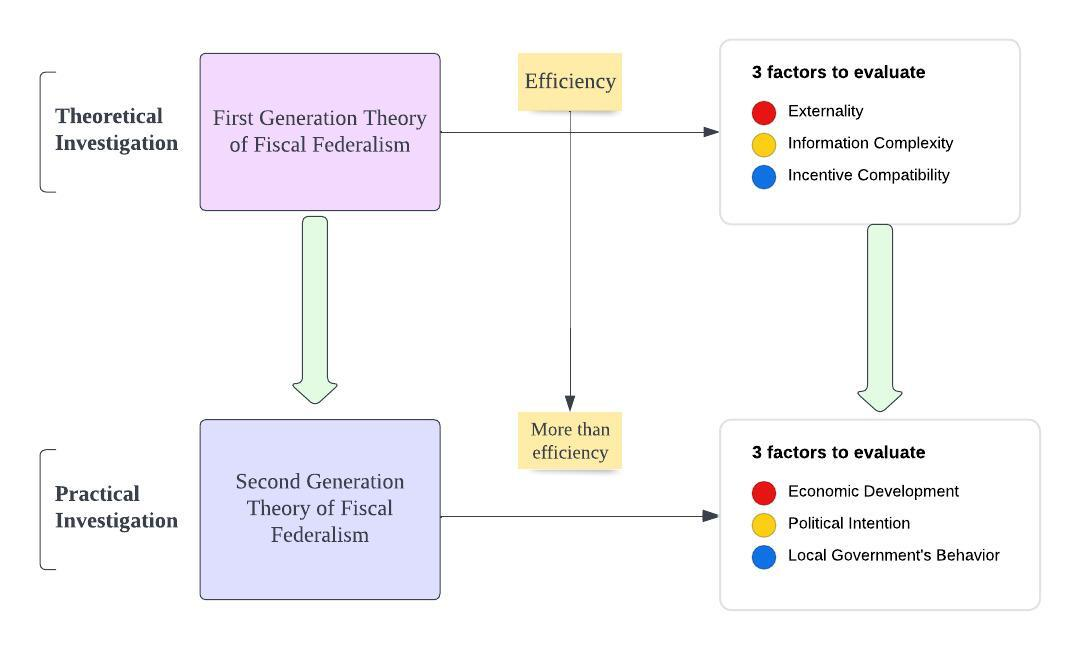
\includegraphics[scale=1]{Chapter-2/Figures/how to evaluate the fiscal federalism.jpeg}
  \caption[How to evaluate the fiscal federalism]{How to evaluate the fiscal federalism
    \texttt{} }
  \label{Figure 1.2}
\end{figure}

In summary, as depicted in Figure \ref*{Figure 1.2}, the original research on fiscal federalism constructed a theoretical framework for efficiently providing public goods. In developed countries, particularly in America, scholars have discovered empirical evidence supporting the advantages of this decentralized fiscal structure. However, in developing countries, fiscal federalism has not worked as effectively, leading to the emergence of second-generation theory. This newer approach focuses on the other side of the coin.


\section{Fiscal Federalism Structure in America}
\subsection{Revenue and Responsibilities of different levels governments}
The United States constitution stipulated that states keep the remaining rights, which means except for the clear defined rights that federal government have, states government keep the undefined rights. Besides, the constitution set no instruction about the responsibilities between state and local governments. This feature combined with the fact that America is a huge country with rich diversity lead to an interesting administrative fact: the responsibilities of state governments in each states are not identical. Within each states, the local governments form up their responsibilities based on the actual needs, thus the local governments are not identical neither. Thus the follow introduction are not describing the administrative reality precisely, but are introducing the general structure.

Under current fiscal federalism system in America, federal, state and local governments rely on different source of income, have different function in supplying the public good and federal government reimburse the state and local government through intergovernmental transfer. On revenue side, from the breakdown of the source of revenue of fiscal year 2019, 50\% of the federal revenue comes from the individual income tax, 7\% from corporate income tax, 36\% is social insurance or payroll tax. On the other hand, on state and local level, intergovernmental transfer accounts for more than 30 percent on average, followed by sales taxes and property tax.\footnote[1]{Data Source:The Department of the Treasury and the Bureau of the Fiscal Service}

\begin{figure}[htbp]
  \centering
  \subfigure[Source of Federal Revenue]{
    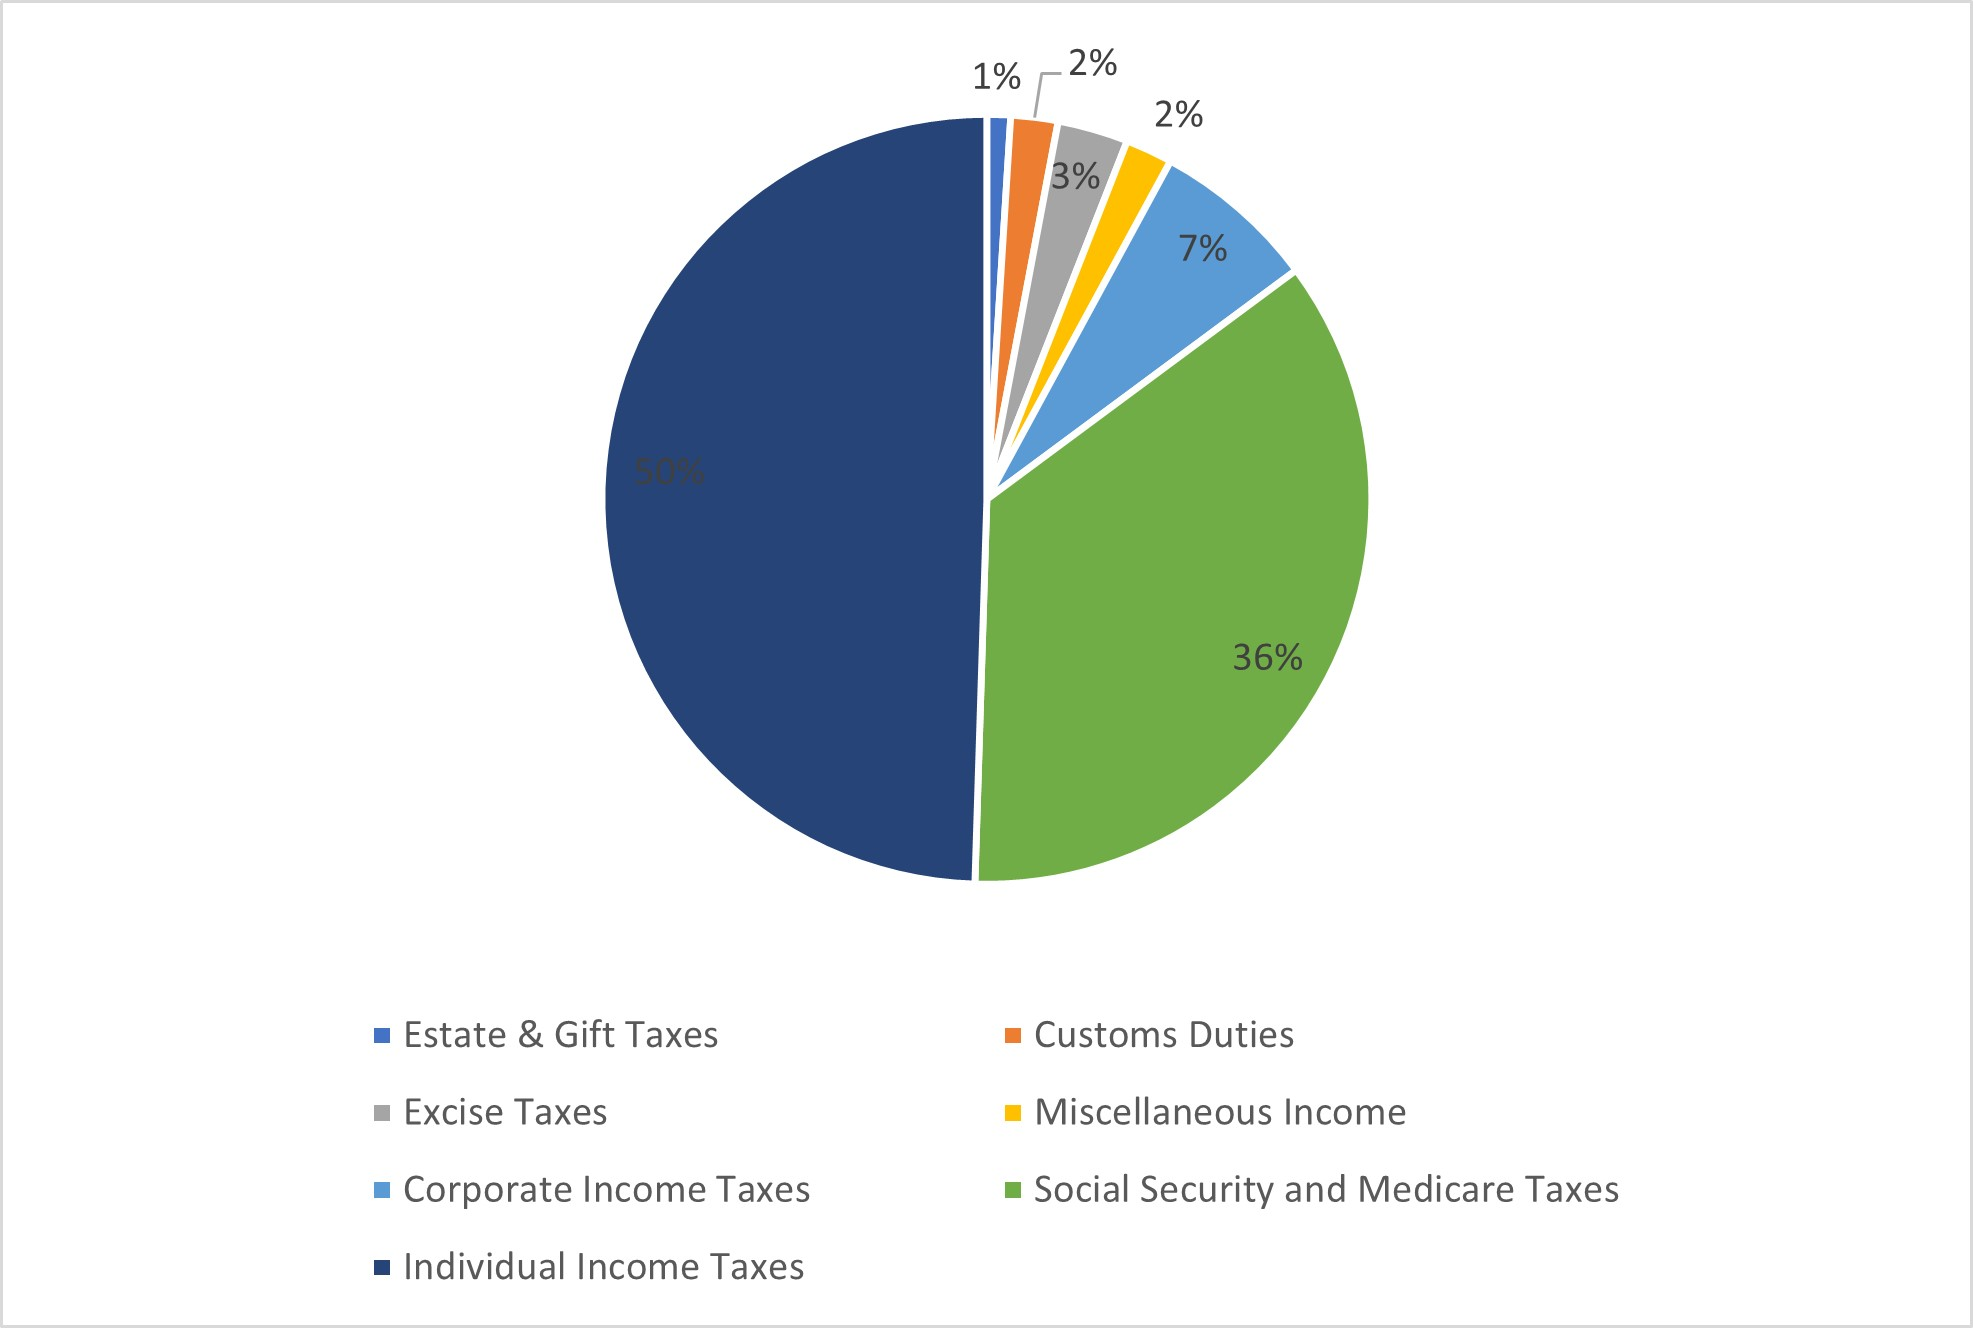
\includegraphics[width=0.31\textwidth]{Chapter-1/Figures/source of federal general revenue.jpg}}
  \subfigure[Source of State Revenue]{
    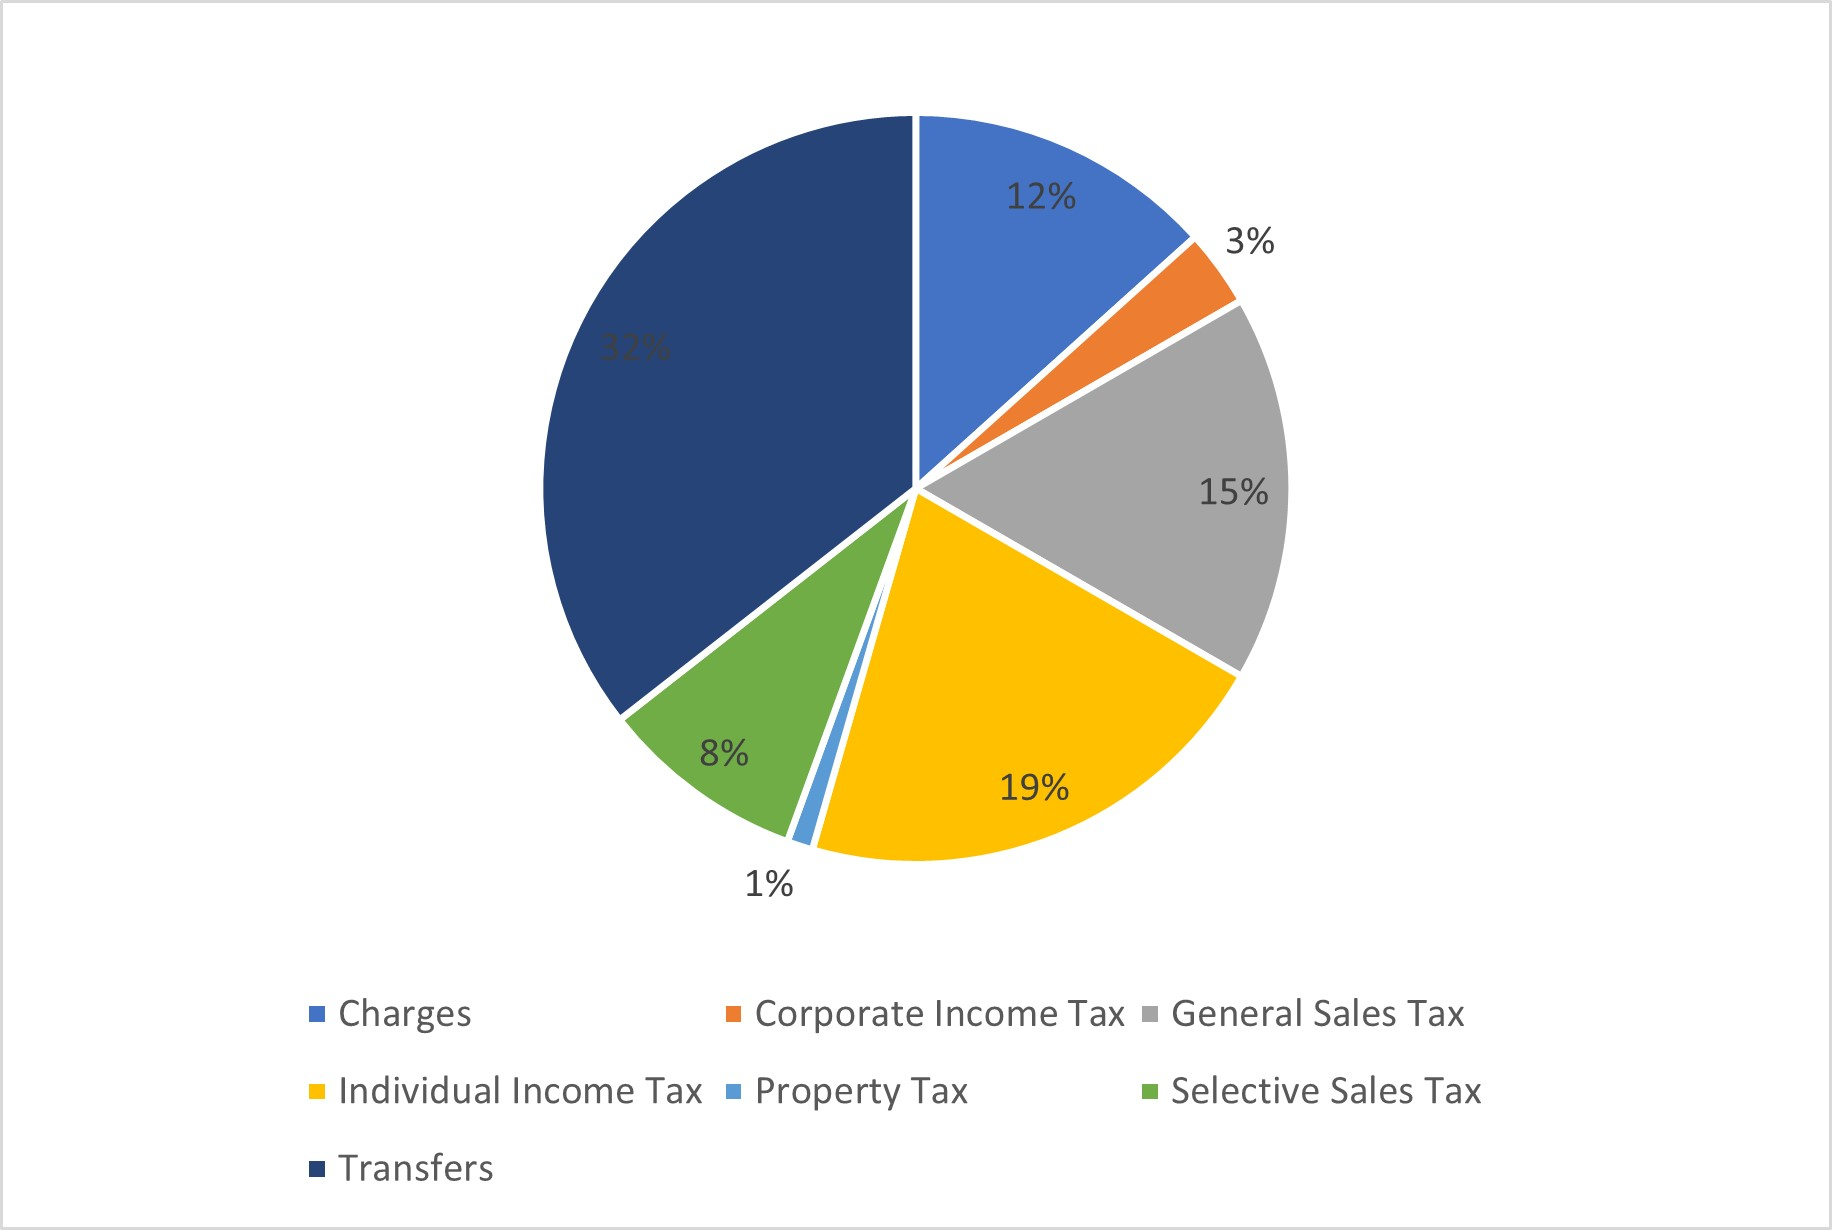
\includegraphics[width=0.31\textwidth]{Chapter-1/Figures/source of state general revenue.jpg}}
  \subfigure[Source of Local Revenue]{
    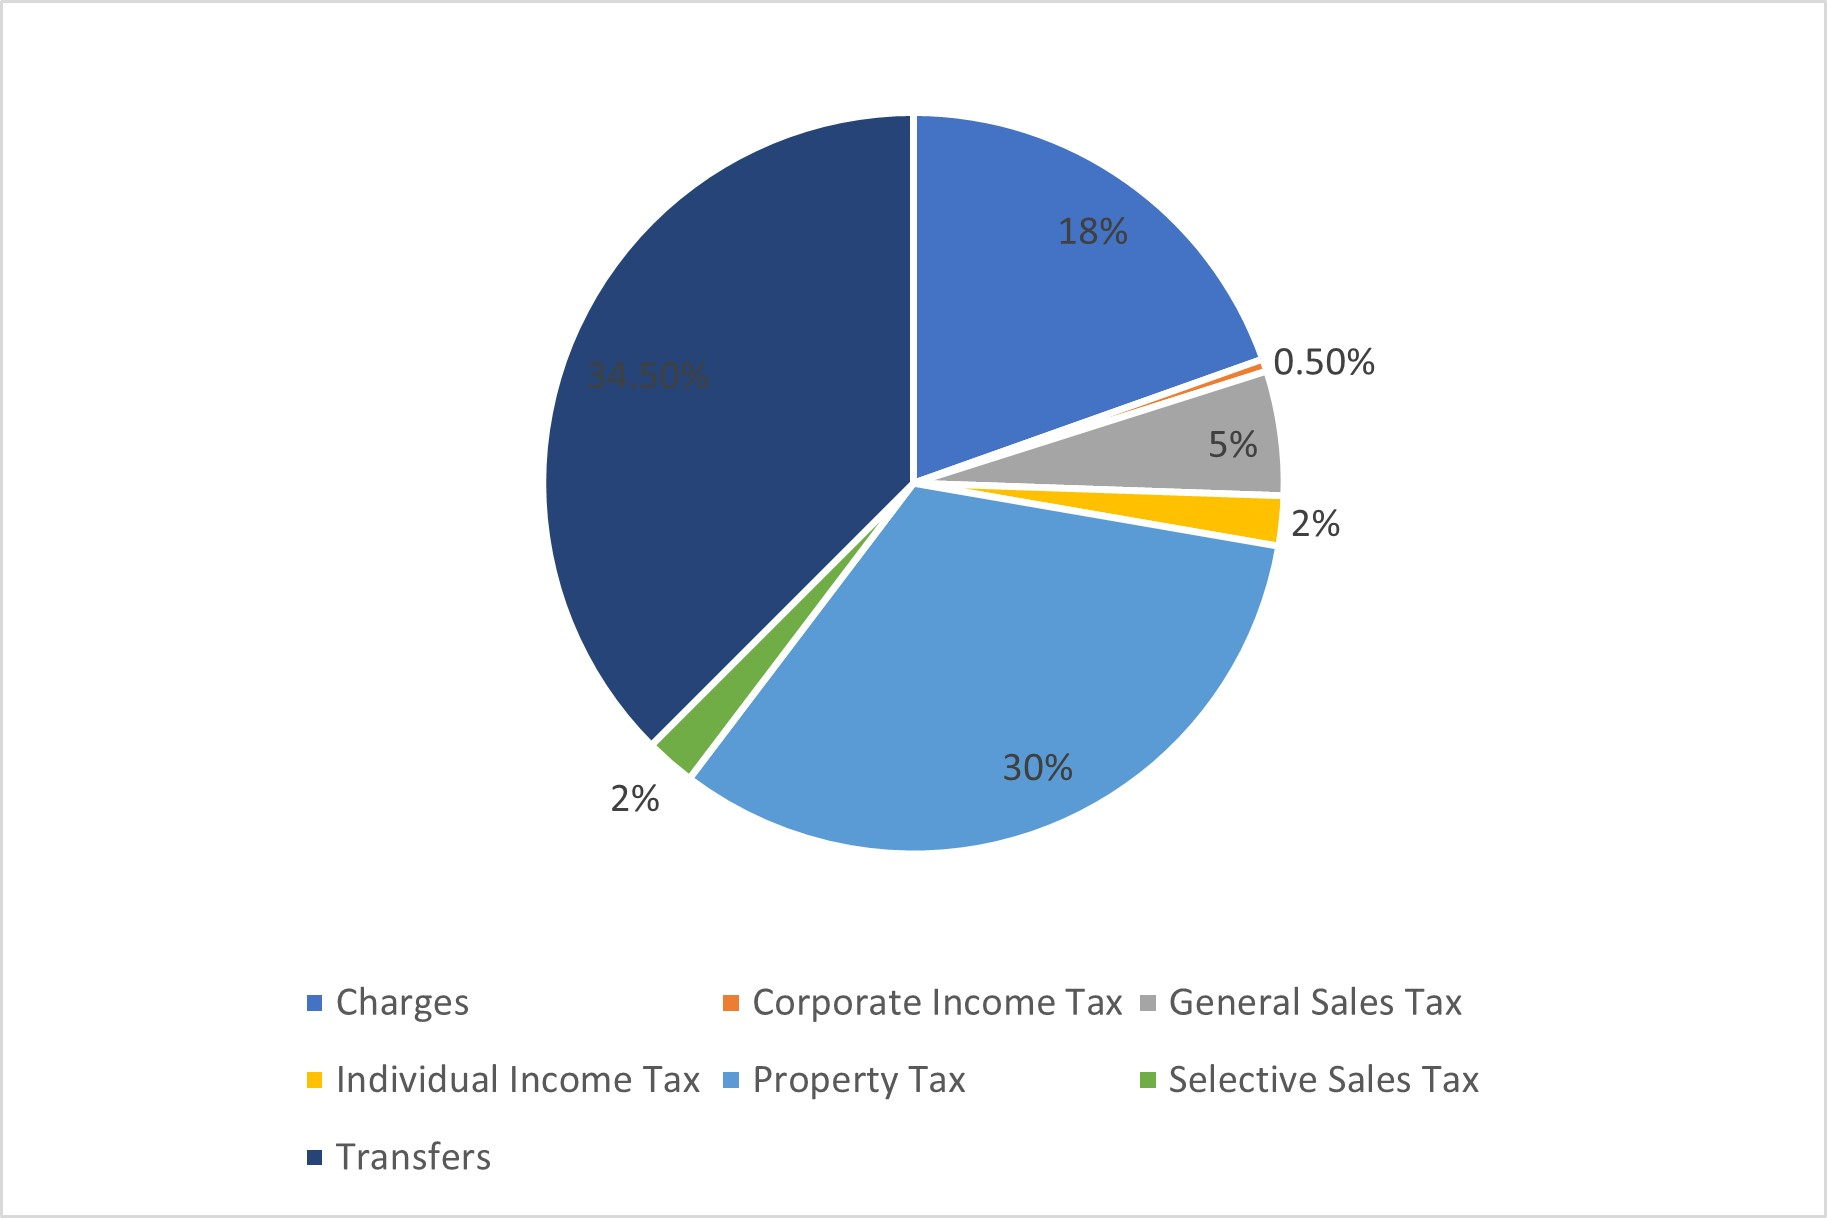
\includegraphics[width=0.31\textwidth]{Chapter-1/Figures/sources of local general revenue.jpg}}
  \caption[Source of Revenue for Multiple Level of Governments in 2019]
  {Source of Revenue for Multiple Level of Governments}
  \label{sourceofreveune}
\end{figure}





%%%
%\begin{figure}[htb]
%    \centering
%    \includegraphics[scale=1]{Chapter-1/Figures/Revenue breakdown of United States}
%    \caption[Revenue breakdown of the different levels of governments in 2019.]{Revenue breakdown of the different levels of governments in 2019.
%    \texttt{Source: U.S. Census of Bureau} }
%    \label{Ch1-figure: Revenue breakdown of United States}
%\end{figure}
%%%

On the expenditure side, federal, state and local government functions differently in supplying public goods and services. Filtered out the public-goods-unrelated expenditure such as interest from debt, federal government is paying for income security, social security, health, national defense, highways and infrastructure, medic care, social services such as education, training and employment. Similarly, if filtered out the expenditure which are unrelated to the public goods and services in state and local governments, the left parts include public welfare, elementary and secondary education, higher education, health and hospitals, highways and roads, police, courts, housing and community development.\footnote[2]{Data Source:The Department of the Treasury and the Bureau of the Fiscal Service }
%%%
%%%%%%%%%%%%%%%%%%%%%%%%%%%%%%%%%%
\begin{figure}[H]
  \centering  %居中
  \subfigure[Federal Expenditure]{   %first subfigure
    \begin{minipage}{7cm}
      \centering    %子图居中
      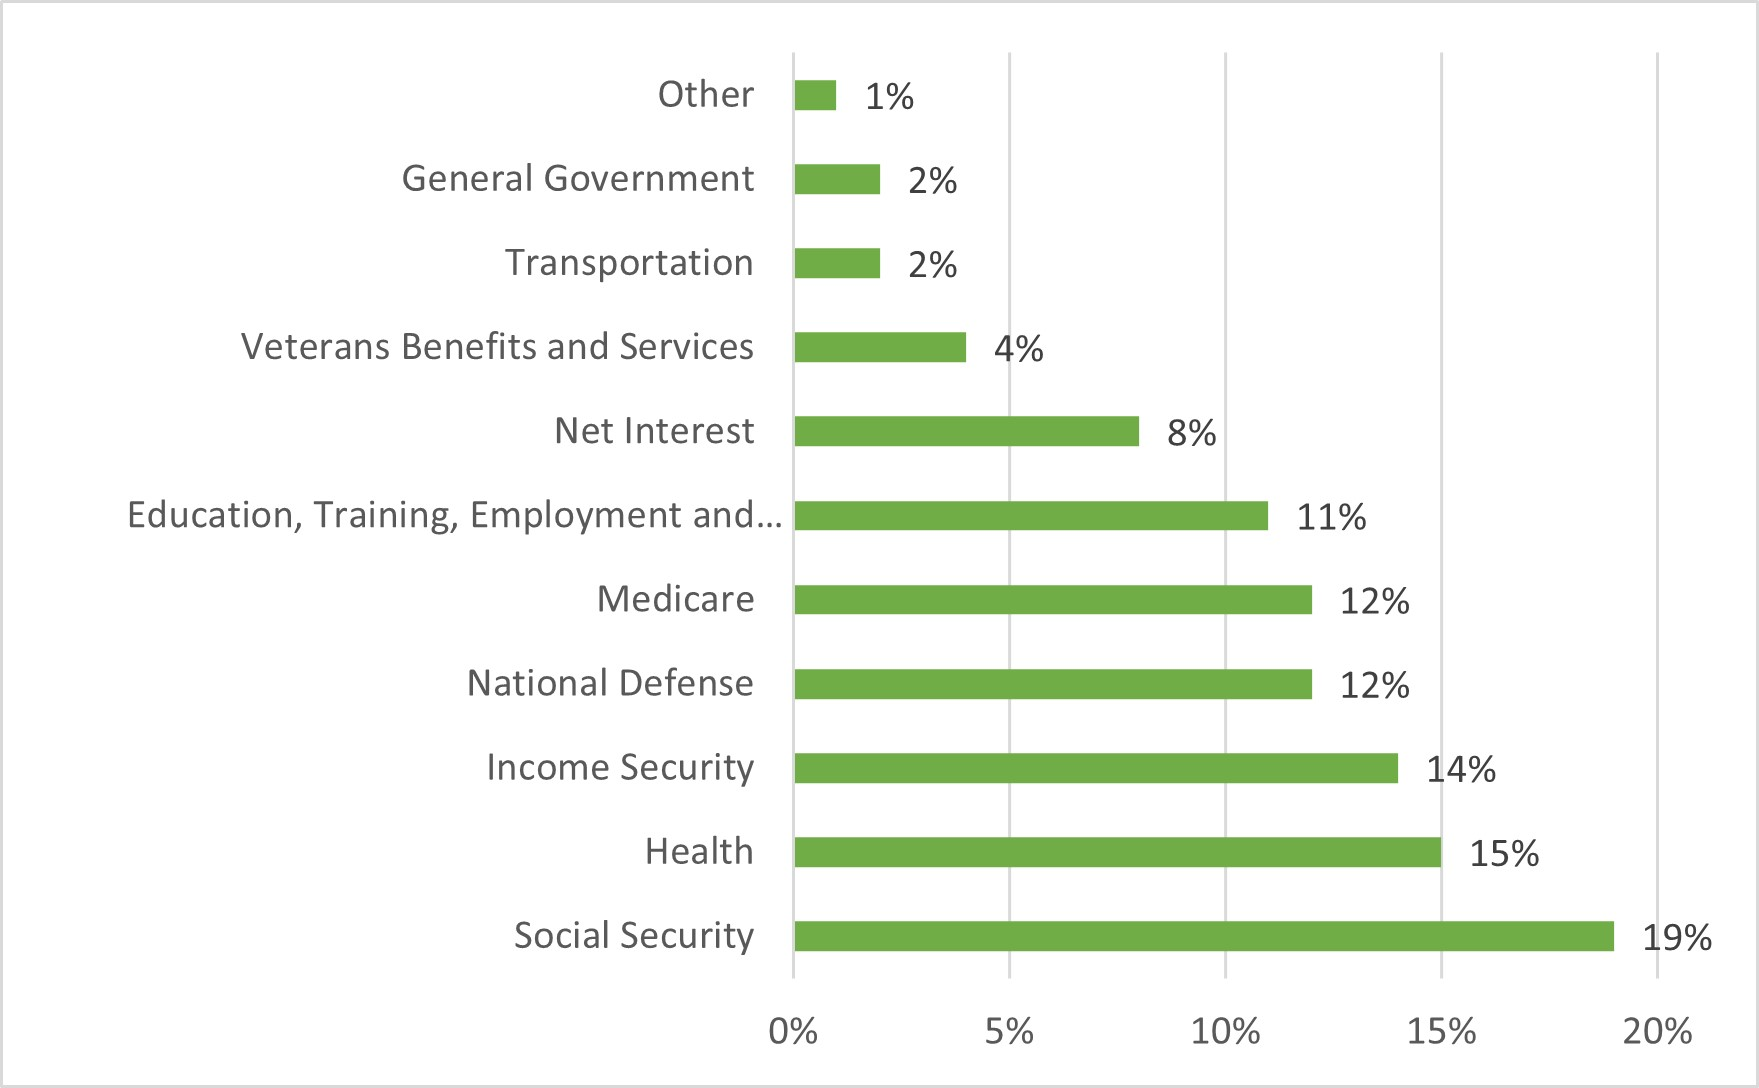
\includegraphics[scale=0.52]{Chapter-1/Figures/federal expenditure.JPG}  %以pic.jpg的0.5倍大小输出
    \end{minipage}
  }
  \subfigure[State and Local Expenditure]{ %second subfigure
    \begin{minipage}{7cm}
      \centering    %子图居中
      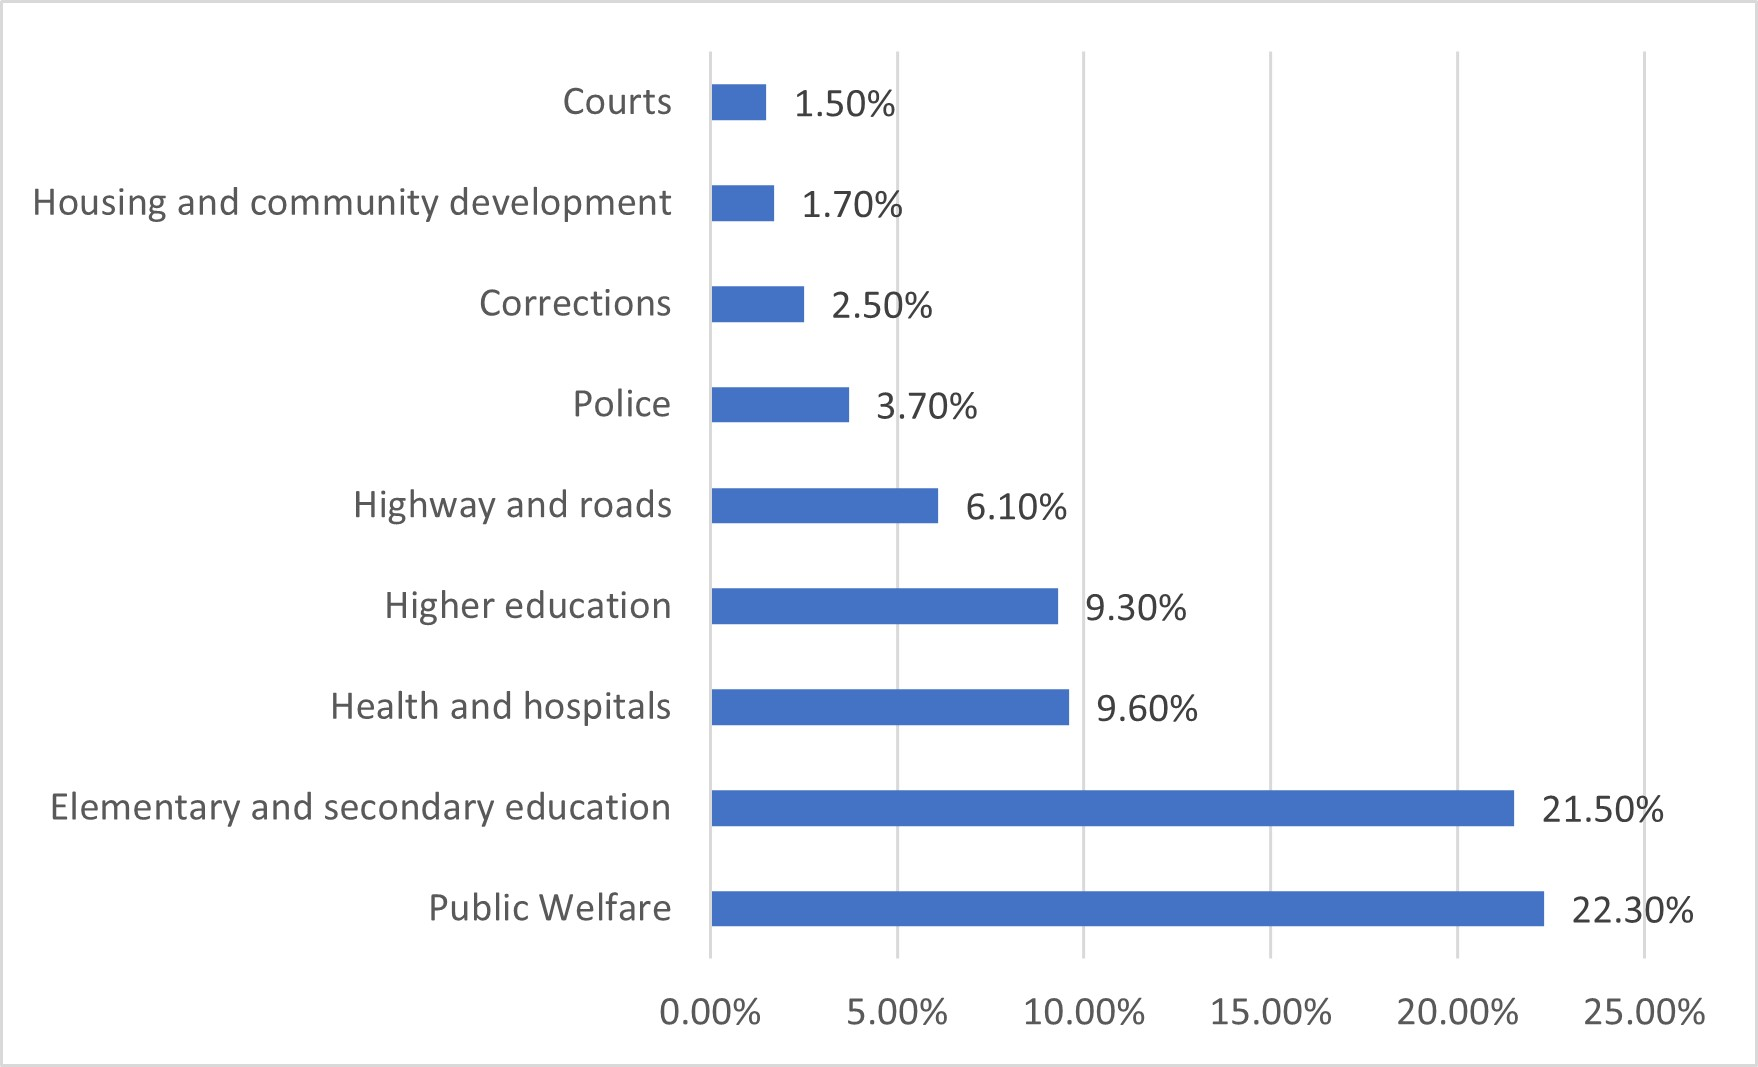
\includegraphics[scale=0.52]{Chapter-1/Figures/state and local expenditure.JPG}%以pic.jpg的0.5倍大小输出
    \end{minipage}
  }

  \caption[Expenditure Structure for Multiple Level of Governments in 2019]{Expenditure Structure for Multiple Level of Governments.}    %caption for whole figure
  \label{Figure 1.3}
\end{figure}

Though the revenue and expenditure structure of federal, state and local government are relatively stable. Figure\ref*{Figure 1.3} shows a cross-sectional data of 2019. A time series fluctuation is presented in Figure\ref*{Figure A.1} attached in Appendix A. Information in Figure\ref*{Figure A.1} shows that it's not a big deal to capture the revenue structure by just breakdown the data in one year.

Federal, state and local government has their unique function in supplying public goods, for example, the federal government is supplying national defense exclusively, while state and local government is the sole supplier in police, courts, housing and community development. Meanwhile, some of the areas are overlapped by both layers of governments, such as public welfare, education, health, highway and infrastructure construction.

\begin{figure}[H]
  \centering
  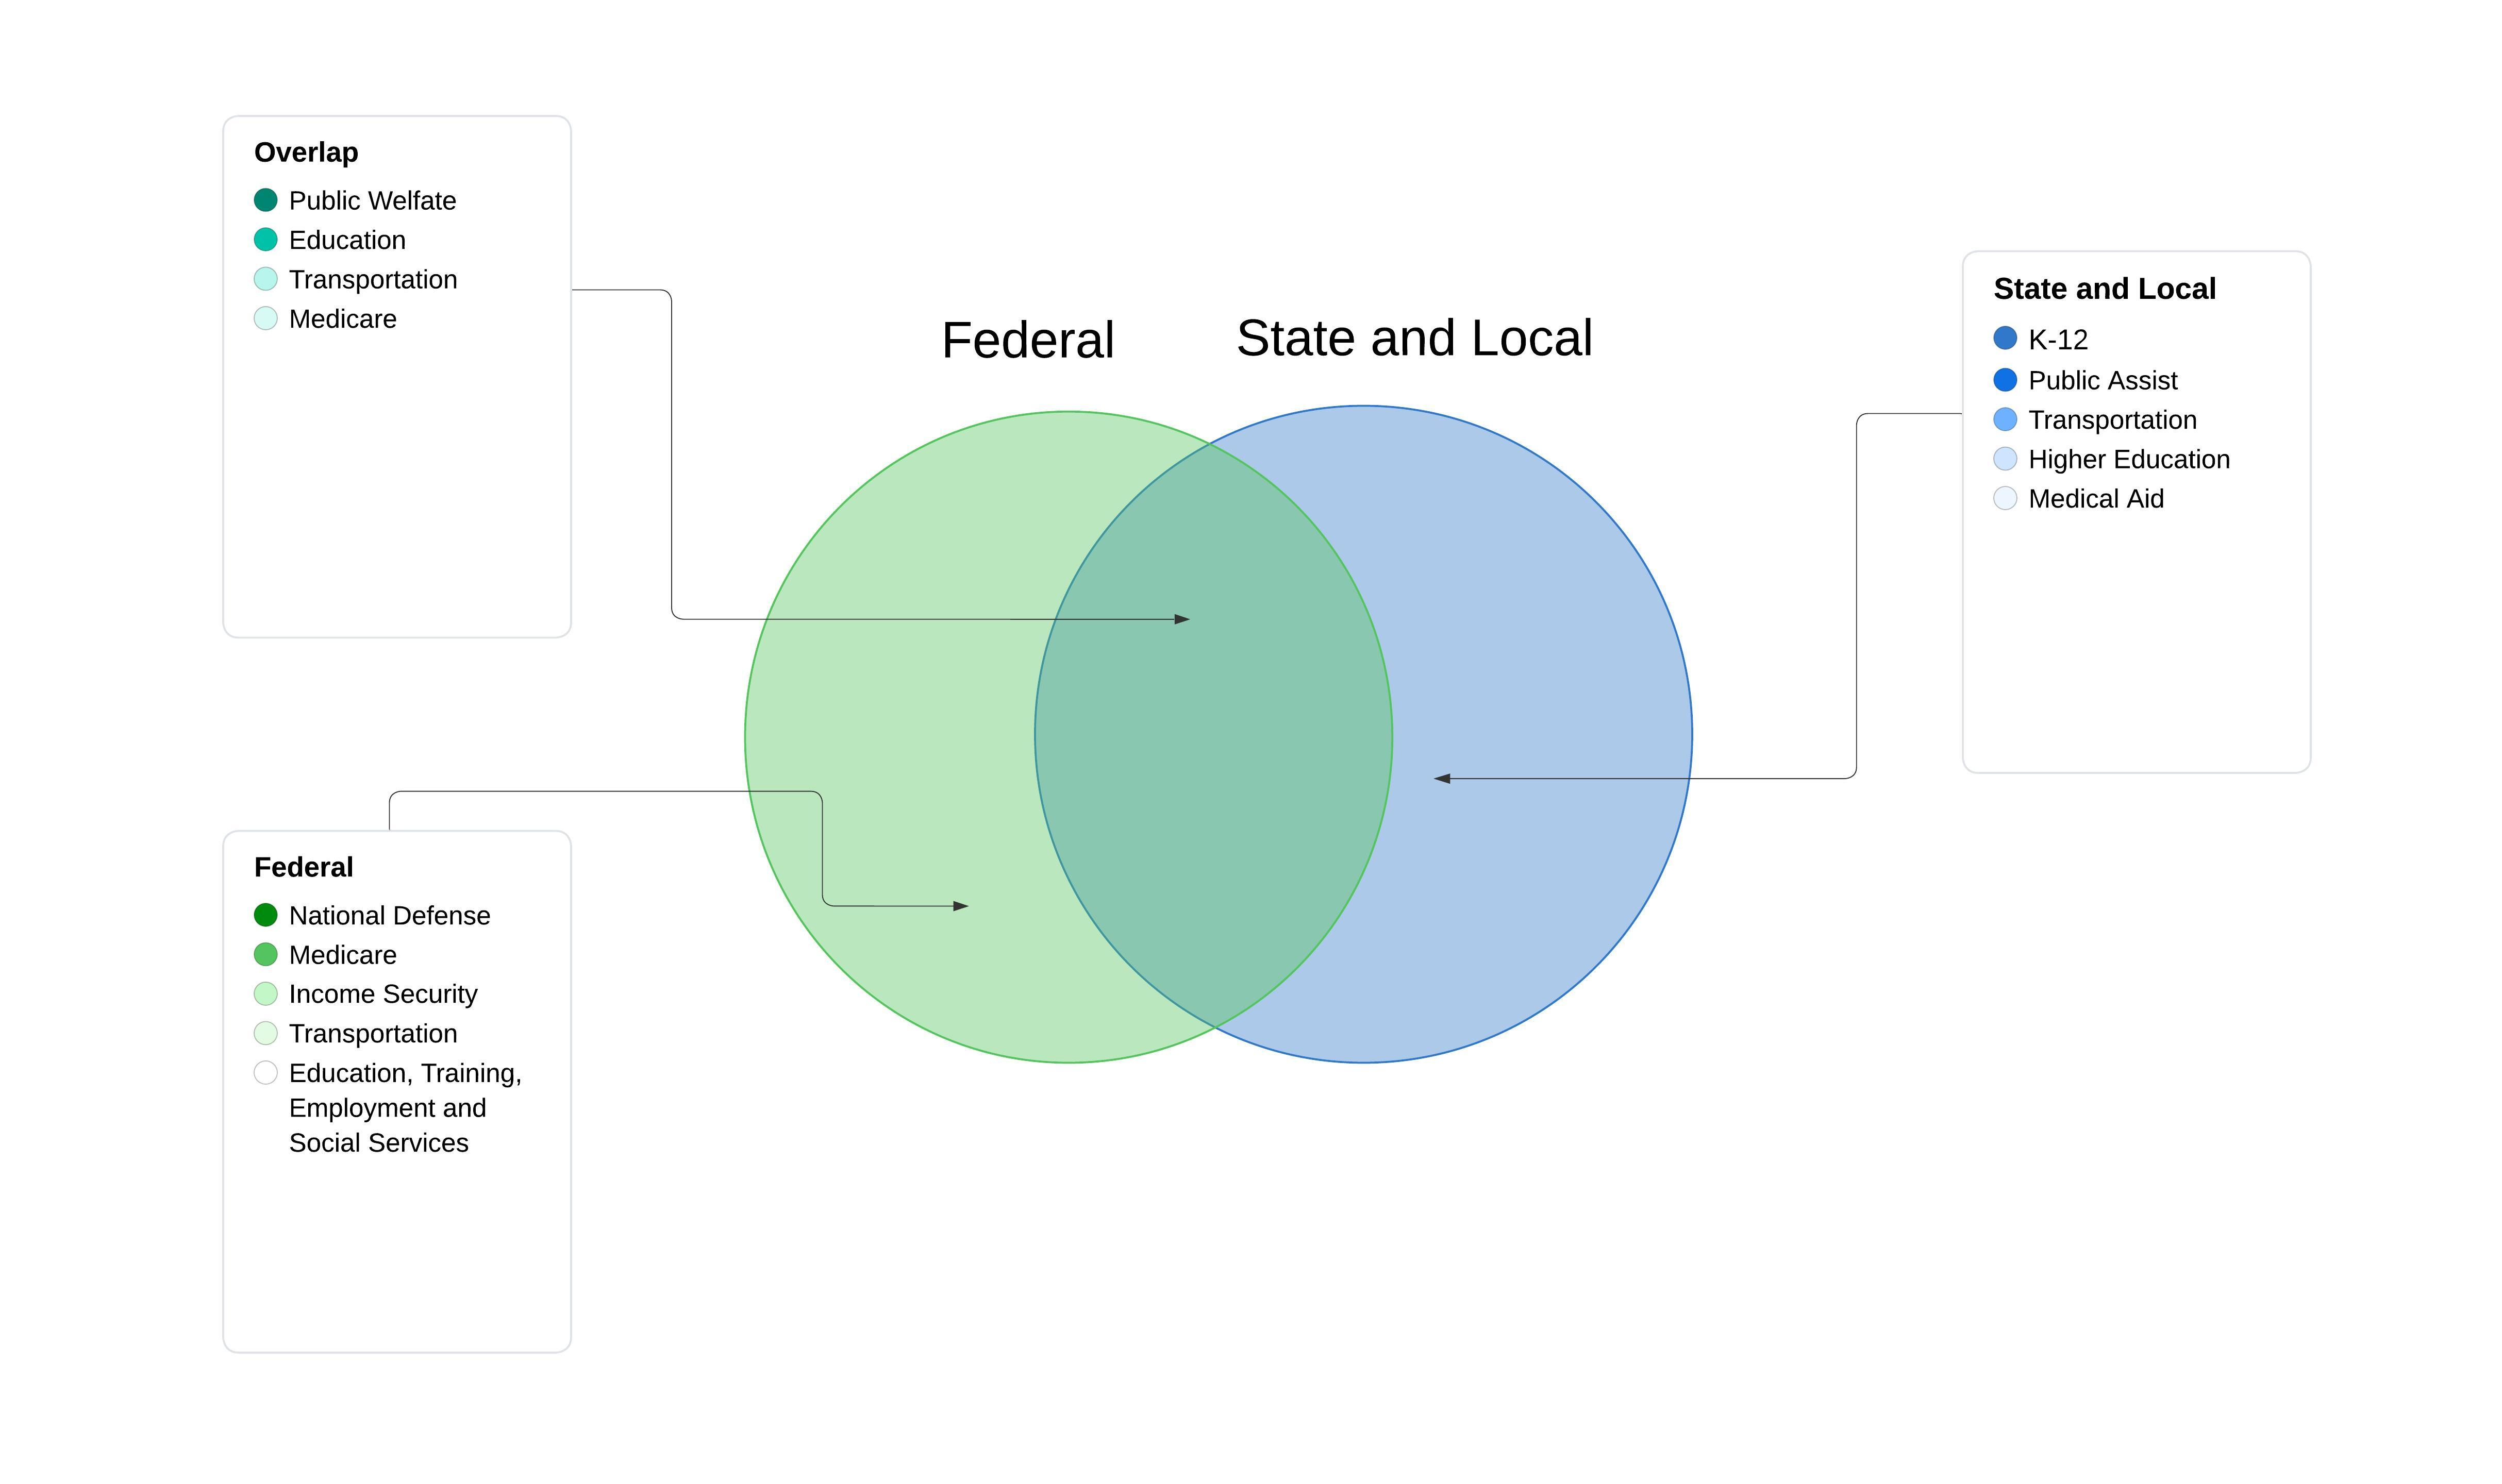
\includegraphics[scale=0.4]{Chapter-1/Figures/Venn graph on public goods.jpeg}
  \caption[Venn graph on public goods and services supplying]{Venn graph on public goods and services supplying by federal, states and local government
    \texttt{} }
  \label{Figure 1.4}
\end{figure}

\subsection{Interaction between National Government and Subnational Governments}
Typically, national governments engage in public goods provision at the subnational level through two approaches: joint provision and intergovernmental transfers. The distinction lies in whether the national government directly provides the public goods. This section delineates and contrasts these two methods.

In the US fiscal federal system, the Federal government imposes significant influence on state and local fiscal decision making through various grants-in-aids programs (GIA) or intergovernmental transfer(IGT). Annually, these programs amounts to nearly \$700 billion, or close to 20 percent of overall federal revenues \cite{dilger2015federal}. Grounded in fiscal federalism, these programs, are guided by the idea that the allocation of publicly funded goods and services should be the responsibility of state and local governments, due to their closer proximity to the constituents. The sought for advantages of such division include: reduced costs associated with planning and administration, the ability to account for spatial differences, and increased opportunities for citizens to influence political decision-making \cite{musgrave1997devolution}. IGT from federal government help to narrow the gap between revenue and expenditure of state and local government, encourage the supply of specific public goods and promote the horizontal equity among states.

Generally, grants-in-aids programs in the US federal fiscal system, can be categorized across two dimensions including the level of restrictions that are attached to the awards, and the administrative procedures that govern the award process. In terms of restrictions, IGT can be organized into categorical grants, block grants and general revenue sharing grants. Categorical grants include formula categorical grants, open-ended reimbursement categorical grants and project categorical grants.Project categorical grants are awarded with relatively strict set of activities that are attached to a specific purpose. Block grants are awarded to fund specific programs, but carry relatively few restrictions. The main difference is that block grants do not attach a specific purpose to how recipients spend the award. General revenue sharing grants carries the least amount of restrictions. In brief, these awards can be spent for any purpose, as long as it is not prohibited by federal or state law.  According to the Congressional Research Service report \cite{dilger2015federal}, there are about 600 grant-in-aid programs, and categorical grants account for about 95 percent of the programs and more than 80 percent of total grant outlays.

% Table generated by Excel2LaTeX from sheet 'Sheet1'
\begin{table}[H]
  \centering
  \caption{Divide Grants by level of Restriction Attached}
  \begin{tabular}{ccc}
    \toprule
    \multicolumn{3}{c}{Level of Restriction}                                   \\
    \midrule
    Low Restriction           & Medium Restriction & High Restriction          \\
    \midrule
    Formula Categorical Grant & Block Grant        & Project Categorical Grant \\
    Open-ended Reimbursement  &                    &                           \\
    General Revenue Sharing   &                    &                           \\
    \bottomrule
  \end{tabular}%
  \label{Table 1.3}%
\end{table}%


In terms of the administrative procedures that govern the awards, the grants can be categorized into three kinds including projects grants \(or competitive grants\), formula grants, and reimbursement grants. For competitive grants, states should apply by submitting a request and get the grants through a competitive process. They are intended to improve the efficiency of funding allocation by encouraging grantees to seek funds for well-planned and exemplary projects. Formula grants are distributed to states through mathematical formulas decided by social characters within the jurisdiction. Typically the factors in the formula depends on the intention of the grants, and common factors may include population, poverty level, income per capita, unemployment rate, enrollment in public schools, etc. Finally, reimbursement grants awards state and local governments in the form of a reimbursement for a specific percentage of state and local spending on a program.The reimbursement amount does not carry a specific limit. Reimbursement grants could be divided into open and closed ended reimbursement grants. The matching mechanism in reimbursement grants is a very intriguing consideration in public economic literature when evaluating the distortion effect. For matching grants, federal governments will reimburse a specific ratio for each 1 dollar of state and local expenditure. Based on whether federal government set a cap on the matching grants, matching grants can be divided into open-ended matching grants and closed-ended grants.

% Table generated by Excel2LaTeX from sheet 'Sheet2'
\begin{table}[htbp]
  \centering
  \caption{Divide Grants by Form of Administrative Procedure}
  \begin{tabular}{clc}
    \toprule
    \multicolumn{3}{c}{Form of Administrative Procedure}                                                                                                     \\
    \midrule
    \multicolumn{1}{p{9.645em}}{ Submitting Request} & \multicolumn{1}{p{10.285em}}{               By Formula} & \multicolumn{1}{p{10.855em}}{Reimbursement} \\
    \midrule
    \multicolumn{1}{l}{Competitive Grants}           & Formula grants                                          & Project Categorical Grant                   \\
                                                     & Formula-project grants                                  &                                             \\
    \bottomrule
  \end{tabular}%
  \label{Table 1.4}%
\end{table}%

In the joint provision process, unlike intergovernmental transfers, national government is the direct provider for part of the public goods in subnational jurisdictions. Such cases wildly exist in those projects under Interstate Maintenance Program, the National Highway Program, the Surface Transportation Program, the Highway bridge Replacement and Rehabilitation Program, the Congestion Mitigation and Air Quality Control Program. The mechanism of joint provision is relatively straight forward, national government collect revenue and supply the public goods directly.

\section{Introduction of the Structure in the Following Chapters}
The objective of this paper is to comprehensively analyze the fiscal federalism structure by addressing a series of questions on national and subnational level. Game theory tools are used to provide a theoretical explanation of fiscal behavior of national and subnational governments in the public goods provision process and theories are empirically tested, with a focus on the American context. Since fiscal federalism involves at least two layers of government, the analysis is conducted by separately investigating questions at both central and subnational levels. There are two questions on central level. For one, how national government choose the way to engage in the subnational public goods provision, which means how national governments decide if it should stay outside, join with intergovernmental transfer or provide the public goods directly. For another, since the intergovernmental transfer is the most influential fiscal tool for national government, the grants distribution mechanism is also an important topic. On subnational level, the main focus is the reactive fiscal behavior of subnational government on national government's decision. To be more specific, the discussion can be divided into two categories, one is the reaction of spending behavior, another on is the revenue collection behavior. The resulting $2\times2$ table gives a comprehensive overview of the content of the following chapters, as is shown in Table \ref*{Table 1.5}.

% Please add the following required packages to your document preamble:
% \usepackage{multirow}
\begin{table}[htb]
  \caption{General Setting of the Questions in Fiscal Federalism Analysis}
  \label{Table 1.5}
  \begin{tabular}{|l|ll|ll}
    \cline{1-3}
    \multirow{2}{*}{}                                                                                                                                                                         & \multicolumn{2}{c|}{Layers of Governments} &                                  &     \\ \cline{2-3}
                                                                                                                                                                                              & \multicolumn{1}{c|}{National}              & \multicolumn{1}{c|}{Subnational} &   & \\ \cline{1-3}
    \begin{tabular}[c]{@{}l@{}}Spending Side \end{tabular}                                                                                                                                    &
    \multicolumn{1}{l|}{\begin{tabular}[c]{@{}l@{}}1.How national government's engaging\\ way is decided? \\ 2.How IGT distribution decision is \\made in national government ?\end{tabular}} &
    \begin{tabular}[c]{@{}l@{}}3.What's the spending reaction of\\ subnational government on IGT?\end{tabular}                                                                                &
                                                                                                                                                                                              &
    \\ \cline{1-3}
    \begin{tabular}[c]{@{}l@{}}Revenue Side\end{tabular}                                                                                                                                      &
    \multicolumn{1}{l|}{\begin{tabular}[c]{@{}l@{}}\end{tabular}}                                                                                                                             &
    \begin{tabular}[c]{@{}l@{}}4.What is the revenue collection \\ reaction of subnational government \\ on IGT?\end{tabular}                                                                 &
                                                                                                                                                                                              &
    \\ \cline{1-3}
  \end{tabular}
\end{table}


Questions about central government, which are questions on the left side in Table \ref*{Table 1.5} will be investigated in two chapters, in which I will talk about the decision making process about engaging method on central level, and how a intergovernmental transfer decision is made in reality. Questions about local government on the right side are included in other chapters. In chapter 4, I'll analyze and describe the spending behavior of subnational governments once they received the intergovernmental transfer from national level. In chapter 4, I'll investigate the revenue collection behavior when subnational governments got the IGT support. For each questions, both theoretical inference and empirical evidence is supplied.






